\documentclass[conference]{IEEEtran}
\IEEEoverridecommandlockouts

\usepackage{cite}
\usepackage{amsmath,amssymb,amsfonts}
\usepackage{algorithmic}
\usepackage{graphicx}
\usepackage{textcomp}
\usepackage{xcolor}
\usepackage{booktabs}
\usepackage{multirow}
\usepackage{pifont}   % for \ding{51} checkmark
\usepackage{tikz}
\usetikzlibrary{arrows.meta, positioning}

\newcommand{\cmark}{\ding{51}}  % checkmark symbol

\def\BibTeX{{\rm B\kern-.05em{\sc i\kern-.025em b}\kern-.08em
    T\kern-.1667em\lower.7ex\hbox{E}\kern-.125emX}}

% ---------------------------------------------------------------
% TikZ styles  --  align=center is critical to allow \\ in nodes
% ---------------------------------------------------------------
\tikzset{
  fbox/.style={rectangle, draw, fill=blue!12, rounded corners=2pt,
               align=center, minimum height=1.8em, minimum width=3.5cm,
               font=\scriptsize},
  cbox/.style={rectangle, draw, fill=orange!18, rounded corners=2pt,
               align=center, minimum height=1.8em,
               font=\scriptsize},
  sbox/.style={rectangle, draw=gray!60, fill=gray!8, rounded corners=2pt,
               align=center, minimum height=1.8em, minimum width=1.6cm,
               font=\scriptsize},
  marr/.style={-{Stealth[length=3.5pt]}, semithick}
}

\begin{document}

% ---------------------------------------------------------------
% TITLE
% ---------------------------------------------------------------
\title{ModalIn: Decentralized P2P Micro-Lending with On-Chain Reputation
Using Soulbound Tokens and Social Trust Primitives for Indonesian MSMEs}

% ---------------------------------------------------------------
% AUTHORS
% ---------------------------------------------------------------
\author{
  \IEEEauthorblockN{Abednego Zebua}
  \IEEEauthorblockA{
    \textit{Dept.\ of Electrical Engineering}\\
    \textit{Computer Engineering Program, Universitas Indonesia}\\
    Depok, Indonesia\\
    abednego.zebua@ui.ac.id}
  \and
  \IEEEauthorblockN{Calvin Wirathama Katoroy}
  \IEEEauthorblockA{
    \textit{Dept.\ of Electrical Engineering}\\
    \textit{Computer Engineering Program, Universitas Indonesia}\\
    Depok, Indonesia\\
    calvin.wirathama@ui.ac.id}
  \and
  \IEEEauthorblockN{Wilman Saragih Sitio}
  \IEEEauthorblockA{
    \textit{Dept.\ of Electrical Engineering}\\
    \textit{Computer Engineering Program, Universitas Indonesia}\\
    Depok, Indonesia\\
    wilman.saragih@ui.ac.id}
}

\maketitle

% ---------------------------------------------------------------
% ABSTRACT
% ---------------------------------------------------------------
\begin{abstract}
Indonesia's 64 million micro, small, and medium enterprises (MSMEs) contribute
61\% of national GDP yet face a credit gap exceeding Rp~2,800~trillion annually
due to the absence of verifiable credit history and physical collateral. Existing
decentralized finance (DeFi) platforms fail this population because they require
overcollateralization in crypto assets. We present ModalIn, an Ethereum-based
peer-to-peer micro-lending decentralized application (DApp) that replaces
physical collateral with a triple-layer on-chain reputation system. ModalIn
issues each borrower a non-transferable Soulbound Token (SBT) as a persistent
digital credit identity, organizes borrowers into tiered Credit Guilds that
formalize Indonesia's collective accountability culture, and enables ETH-staked
peer vouching as social guarantee. A composite reputation score weighted 50\%
payment history, 30\% vouch score, and 20\% oracle attestation drives an
algorithmic annual percentage rate (APR) model bounded between 6\% and 36\%
in alignment with Indonesian Financial Services Authority (OJK) reference
bounds. The system comprises six interacting Solidity smart contracts deployed
on the Ethereum Sepolia testnet, validated by 29 passing test scenarios. Results
show that a Gold-tier, high-reputation borrower achieves an APR as low as 6\%
compared to 17\% for an unscored borrower, a reduction of up to 65\%, and a
threefold improvement over typical informal moneylender rates.
\end{abstract}

\begin{IEEEkeywords}
blockchain, soulbound token, decentralized finance, micro-lending,
credit scoring, peer-to-peer lending, smart contract, MSME
\end{IEEEkeywords}

% ---------------------------------------------------------------
% I. INTRODUCTION
% ---------------------------------------------------------------
\section{Introduction}

Micro, small, and medium enterprises (MSMEs) form the backbone of Indonesia's
economy. With over 64~million units, they contribute approximately 61\% of
national gross domestic product and absorb 97\% of the domestic
workforce~\cite{b4}. Despite this economic significance, more than 40\% of
Indonesian MSMEs lack access to formal banking credit, creating a financing gap
estimated at over Rp~2,800~trillion per year~\cite{b4}. The root causes are
structural: conventional credit scoring systems require documented repayment
histories and physical assets as collateral, prerequisites that most
informal-sector MSME operators cannot meet~\cite{b3}.

Unable to access formal channels, these businesses resort to informal
moneylenders (\textit{rentenir}) whose annualized interest rates commonly reach
20\%--60\%~\cite{b9}. This creates a vicious cycle: prohibitive interest burden
prevents capital accumulation, which in turn prevents the formation of credit
history needed to qualify for cheaper formal loans.

Blockchain technology offers a structural solution by resolving information
asymmetry between lenders and borrowers without a trusted
intermediary~\cite{b4}. The immutability of on-chain records ensures that
repayment history cannot be manipulated, providing lenders with mathematical
certainty. The Soulbound Token (SBT), a non-transferable, wallet-bound digital
artifact representing commitments and credentials~\cite{b1}, enables a
persistent, unforgeable credit identity that follows a borrower across all
transactions on the network.

Critically, Indonesian informal credit culture already embeds the primitives
needed for reputation-based lending. The \textit{arisan} (rotating savings
group), \textit{koperasi} (cooperative), and \textit{gotong royong} (mutual
aid) traditions demonstrate that collective accountability and social guarantee
are culturally validated mechanisms for reducing default risk. What has been
missing is infrastructure that encodes these social trust mechanisms into
verifiable, immutable on-chain data.

We present \textbf{ModalIn}, a decentralized P2P micro-lending DApp that
translates these cultural trust primitives into smart contract logic on the
Ethereum Virtual Machine (EVM). The contributions of this paper are:

\begin{enumerate}
\item A \textbf{triple-layer on-chain reputation model} combining payment
history, ETH-staked peer vouching, and off-chain oracle attestation into a
composite credit score on a 0--1000 scale, with formal weight assignment and
a time-based reputation decay mechanism.

\item An \textbf{algorithmic interest rate model} computing APR directly from
on-chain reputation and group tier, with OJK-referenced bounds (6\%--36\%),
eliminating manual underwriting.

\item A \textbf{Credit Guild mechanism} (Bronze/Silver/Gold tier) formalizing
\textit{gotong royong} collective accountability as a smart contract primitive
with group-level score propagation.

\item A \textbf{full working DApp}: six Solidity contracts (Hardhat~3.1.12,
OpenZeppelin~v5.6), a React~19 frontend with ethers.js~v6 integration,
deployed on the Ethereum Sepolia testnet, and validated by 29 automated test
scenarios.
\end{enumerate}

% ---------------------------------------------------------------
% II. RELATED WORK
% ---------------------------------------------------------------
\section{Related Work}

\subsection{Overcollateralized DeFi Lending}

Dominant DeFi lending protocols such as Aave and Compound use overcollateral-
ization, requiring borrowers to lock crypto assets worth 120\%--150\% of the
loan value~\cite{b7}. While this protects lenders, it is fundamentally
inaccessible to MSMEs who hold no crypto assets. Goldfinch~\cite{b14}
partially addresses this by introducing off-chain trust anchors, but still
relies on institutional backers rather than individual on-chain reputation.
ModalIn departs from this paradigm entirely: no crypto collateral is required,
and reputation is the sole collateral.

\subsection{Traditional Group Lending}

The Grameen Bank model~\cite{b13} demonstrated that group-based social
pressure can reduce default rates to below 2\% in microcredit populations with
no physical collateral. However, Grameen's model is manual, centralized, and
non-auditable at global scale. ModalIn encodes the same social accountability
mechanism (collective responsibility, tiered trust, and social guarantee) as
immutable smart contract logic.

\subsection{Blockchain for SME Finance}

Kumar et al.~\cite{b4} conducted a systematic review of blockchain-based SME
finance and found strong evidence that distributed ledgers reduce information
asymmetry and transaction costs, but their work remains a literature review
without a system architecture. Kanga et al.~\cite{b3} examined blockchain-based
microcredit platforms in developing countries and identified on-chain identity
as the critical missing component for financial inclusion. Ante et al.~\cite{b7}
analyzed blockchain as a solution for P2P lending fraud, concluding that
immutability addresses the core trust problem but offered no reputation scoring
mechanism. Nanayakkara et al.~\cite{b5} proposed swarm learning for P2P credit
scoring, but their approach relies on off-chain machine learning rather than
on-chain identity primitives.

\subsection{On-Chain Reputation and Soulbound Tokens}

Weyl, Ohlhaver, and Buterin~\cite{b1} introduced Decentralized Society (DeSoc)
and SBTs as non-transferable tokens encoding social relationships and
credentials. EIP-5114~\cite{b12} standardizes the Soulbound Badge interface.
ModalIn operationalizes these concepts specifically for credit scoring with a
weighted multi-dimensional formula. Table~\ref{tab:related} positions ModalIn
against the most closely related systems.

\begin{table}[t]
\caption{Comparison of Related Systems}
\label{tab:related}
\centering
\begin{tabular}{p{1.4cm}p{1.7cm}p{2.2cm}p{1.0cm}}
\toprule
\textbf{System} & \textbf{Mechanism} & \textbf{Key Limitation} & \textbf{Collateral} \\
\midrule
Aave/Compound & Overcollateral   & Excludes unbanked      & Crypto \\
Grameen Bank  & Group lending    & Manual, centralized    & Social \\
Goldfinch     & Off-chain trust  & Institutional backers  & Off-chain \\
Kumar et al.  & Review only      & No architecture        & N/A \\
\textbf{ModalIn} & \textbf{SBT+Guild+Vouch} & \textbf{ETH denomination} & \textbf{Reputation} \\
\bottomrule
\end{tabular}
\end{table}

% ---------------------------------------------------------------
% III. PROPOSED METHOD
% ---------------------------------------------------------------
\section{Proposed Method}

\subsection{Problem Formalization}

Given a borrower $b$ with no prior formal credit record, we seek to compute a
verifiable trust score $S(b) \in [0, 1000]$ derived solely from on-chain
behavior, and use it to determine a fair lending APR:
%
\begin{equation}
\text{APR}(b) = \text{BaseRate} + \text{GroupPremium}(b) - \text{RepDiscount}(b)
\label{eq:apr}
\end{equation}
%
where all terms are in basis points (1~bps $= 0.01\%$), and APR is clamped to
$[\text{APR}_\text{min},\, \text{APR}_\text{max}] = [600,\, 3600]$~bps,
corresponding to 6\%--36\% annually in alignment with OJK reference bounds.

\subsection{Triple-Layer Reputation Model}

The composite credit score aggregates three orthogonal trust signals:
%
\begin{equation}
S(b) = \frac{w_p \cdot P(b) + w_v \cdot V(b) + w_a \cdot A(b)}{100}
\label{eq:score}
\end{equation}
%
where $P(b) \in [0, 1000]$ is the \textbf{payment score} computed as $10r$
with $r = (\text{loans repaid} / \text{loans taken}) \times 100$; $V(b)
\in [0, 1000]$ is the \textbf{vouch score} from ETH-staked peer guarantees
computed by \texttt{VouchRegistry}; $A(b) \in [0, 1000]$ is the
\textbf{attestation score} from an authorized oracle (e.g., e-commerce
transaction data); and weights $w_p = 50$, $w_v = 30$, $w_a = 20$ sum to 100.

The weight assignment reflects the hierarchy of manipulation resistance:
payment history is fully on-chain and hardest to forge; vouching requires
real ETH at stake; attestation carries oracle centralization risk, hence the
lowest weight.

\subsection{Reputation Decay}

To prevent stale high scores from being exploited, a time-based decay applies
a penalty of 10~points per 180-day period of inactivity:
%
\begin{equation}
S_\text{final}(b) = \max\!\left(0,\; S(b) - 10
  \left\lfloor \frac{t_\text{now} - t_\text{last}}{T_\text{decay}}
  \right\rfloor \right)
\label{eq:decay}
\end{equation}
%
where $T_\text{decay} = 180$~days and $t_\text{last}$ is the timestamp of the
last on-chain update stored in the borrower's SBT profile.

\subsection{Social Trust Mapping}

A central design insight of ModalIn is the direct mapping of Indonesian social
trust practices to on-chain primitives, as shown in Table~\ref{tab:mapping}.

\begin{table}[t]
\caption{Indonesian Social Trust to Smart Contract Mapping}
\label{tab:mapping}
\centering
\begin{tabular}{p{1.9cm}p{2.0cm}p{2.0cm}}
\toprule
\textbf{Indonesian Tradition} & \textbf{ModalIn Mechanism} & \textbf{Contract} \\
\midrule
Credit bureau / bank history  & Payment score via SBT & \texttt{SoulboundToken} \\
\textit{Koperasi / Arisan}    & Credit Guild (Bronze/Silver/Gold) & \texttt{GuildSBT} \\
\textit{Jaminan} / guarantee  & Peer vouch + ETH slash & \texttt{VouchRegistry} \\
Merchant sales data           & Attestation oracle     & \texttt{ReputationEngine} \\
Loan escrow                   & P2P lifecycle          & \texttt{LoanEscrow} \\
\bottomrule
\end{tabular}
\end{table}

% ---------------------------------------------------------------
% IV. SYSTEM DESIGN
% ---------------------------------------------------------------
\section{System Design}

\subsection{Architecture Overview}

ModalIn adopts a strict separation-of-concerns architecture across two layers,
as shown in Fig.~\ref{fig:arch}. The \textbf{Frontend Layer} is a React~19
web application that communicates through ethers.js~v6 and a MetaMask wallet
extension. All state-changing interactions are submitted as cryptographically
signed transactions; no centralized database stores any loan or reputation
state. The \textbf{Blockchain Protocol Layer} consists of six Solidity
contracts with a defined dependency hierarchy: \texttt{LoanEscrow} is the
primary orchestrator, delegating APR computation to
\texttt{InterestRateModel} and reputation updates to
\texttt{ReputationEngine}, which reads from and writes to
\texttt{SoulboundToken}, \texttt{GuildSBT}, and \texttt{VouchRegistry}.

\begin{figure}[t]
\centering
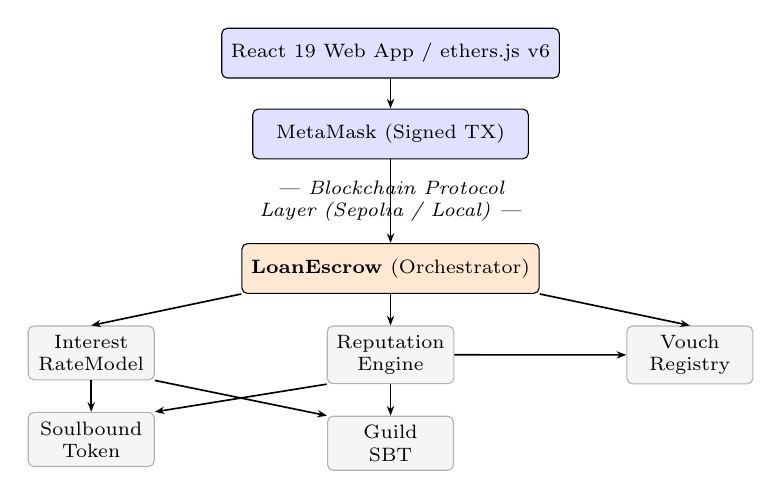
\begin{tikzpicture}[node distance=0.38cm and 0.4cm]
  %% -- Frontend layer --
  \node[fbox] (react) {React~19 Web App / ethers.js v6};
  \node[fbox, below=of react] (mm) {MetaMask (Signed TX)};

  %% -- Layer separator label --
  \node[font=\scriptsize\itshape, below=0.15cm of mm,
        text width=3.5cm, align=center] (sep)
    {--- Blockchain Protocol Layer (Sepolia / Local) ---};

  %% -- Main orchestrator --
  \node[cbox, minimum width=3.5cm, below=0.15cm of sep] (escrow)
    {\textbf{LoanEscrow} (Orchestrator)};

  %% -- Second tier --
  \node[sbox, below left=0.4cm and 1.1cm of escrow]  (irm)
    {Interest\\RateModel};
  \node[sbox, below=0.4cm of escrow]                  (re)
    {Reputation\\Engine};
  \node[sbox, below right=0.4cm and 1.1cm of escrow] (vouch)
    {Vouch\\Registry};

  %% -- Third tier --
  \node[sbox, below=0.4cm of irm]   (sbt)   {Soulbound\\Token};
  \node[sbox, below=0.4cm of re]    (guild) {Guild\\SBT};

  %% -- Arrows: frontend --
  \draw[marr] (react)  -- (mm);
  \draw[marr] (mm)     -- (escrow);

  %% -- Arrows: orchestrator to second tier --
  \draw[marr] (escrow.south west) -- (irm.north);
  \draw[marr] (escrow.south)      -- (re.north);
  \draw[marr] (escrow.south east) -- (vouch.north);

  %% -- Arrows: second to third tier --
  \draw[marr] (irm.south)     -- (sbt.north);
  \draw[marr] (irm.south east) -- (guild.north west);
  \draw[marr] (re.south)      -- (guild.north);
  \draw[marr] (re.south west) -- (sbt.north east);
  \draw[marr] (re.east)       -- (vouch.west);
\end{tikzpicture}
\caption{ModalIn two-layer architecture. The frontend communicates exclusively
through signed transactions; all loan and reputation state is stored on-chain.}
\label{fig:arch}
\end{figure}

\subsection{Smart Contract Design}

Table~\ref{tab:contracts} summarizes the six contracts and their
responsibilities. The \texttt{SoulboundToken} stores each borrower's
\texttt{CreditProfile} struct (encompassing loan counts, cumulative amounts,
reputation score, and last-updated timestamp) and starts new borrowers at a
neutral score of 500. The \texttt{GuildSBT} assigns tier based on collective
average score: Bronze ($S < 650$), Silver ($650 \leq S < 800$), Gold
($S \geq 800$). The \texttt{VouchRegistry} records ETH-staked peer guarantees
and slashes stakes proportionally upon borrower default.

\begin{table}[t]
\caption{Smart Contract Summary}
\label{tab:contracts}
\centering
\begin{tabular}{p{1.9cm}p{4.7cm}}
\toprule
\textbf{Contract} & \textbf{Key Responsibility} \\
\midrule
\texttt{Soulbound}\newline\texttt{Token}
  & Non-transferable ERC-5114-inspired credit identity; stores \texttt{CreditProfile}; starting score 500; \texttt{transfer()} permanently reverts. \\[2pt]
\texttt{GuildSBT}
  & Credit group (2--10 members); tier Bronze/Silver/Gold from collective score; tier updates on \texttt{recalculateScore()}. \\[2pt]
\texttt{VouchRegistry}
  & ETH-staked peer vouches; stake-weighted vouch score; slashes on default. \\[2pt]
\texttt{Reputation}\newline\texttt{Engine}
  & Aggregates $S(b)$ per~\eqref{eq:score}; applies decay per~\eqref{eq:decay}; propagates to guild average. \\[2pt]
\texttt{InterestRate}\newline\texttt{Model}
  & APR per~\eqref{eq:apr}: Bronze +800~bps, Silver +400~bps, Gold +0~bps; reputation discount up to $-600$~bps. \\[2pt]
\texttt{LoanEscrow}
  & Loan states: Requested $\to$ Active $\to$ Repaid/Defaulted; holds ETH in escrow; triggers reputation update on resolution. \\
\bottomrule
\end{tabular}
\end{table}

\subsection{Access Control and Security Design}

Sensitive state-writing functions (\texttt{updateReputation},
\texttt{recordLoan}, \texttt{recordRepayment}) are protected by an
\texttt{authorizedUpdaters} whitelist pattern rather than role-based access
control, keeping gas overhead low while preventing unauthorized score
manipulation. All ETH-moving functions (\texttt{fundLoan},
\texttt{repayLoan}, \texttt{withdrawFunds}) are guarded with OpenZeppelin's
\texttt{ReentrancyGuard}. \texttt{LoanEscrow} additionally follows the
Checks-Effects-Interactions (CEI) pattern: all state updates precede external
ETH transfers, eliminating reentrancy vectors by design.

% ---------------------------------------------------------------
% V. IMPLEMENTATION
% ---------------------------------------------------------------
\section{Implementation}

\subsection{Technology Stack}

Table~\ref{tab:stack} lists the exact component versions used in ModalIn.

\begin{table}[t]
\caption{Technology Stack}
\label{tab:stack}
\centering
\begin{tabular}{lll}
\toprule
\textbf{Component} & \textbf{Version} & \textbf{Role} \\
\midrule
Solidity          & 0.8.20   & Smart contract language \\
Hardhat           & 3.1.12   & EVM dev environment \\
OpenZeppelin      & v5.6.1   & Ownable, ReentrancyGuard \\
ethers.js         & v6.16.0  & Frontend--contract bridge \\
React             & 19       & Frontend framework \\
TypeScript        & v5.8.2   & Frontend type safety \\
Vite              & v6.2.0   & Build toolchain \\
TailwindCSS       & v4.1.14  & UI styling \\
Mocha / Chai      & 11.x / 6.x & Test runner / assertions \\
Node.js           & v24.11.1 & Runtime environment \\
\bottomrule
\end{tabular}
\end{table}

\subsection{Deployment Strategy}

Two deployment environments are supported. For local development,
\texttt{hardhat node} instantiates a simulated EVM (Chain~ID~31337) with
controllable block timestamps, enabling testing of deadline and decay
scenarios. The deploy script deploys all six contracts in dependency order and
injects their addresses into
\texttt{modalin-frontend/src/abis/contract-addresses.json}, making the
frontend environment-agnostic. For public validation, contracts were deployed
to the \textbf{Ethereum Sepolia testnet} (Proof of Stake) using
\texttt{deploy:sepolia}, demonstrating viability with real consensus and block
finality.

\subsection{Key Implementation Decisions}

\textbf{Basis-point APR arithmetic.} Solidity does not support floating-point.
All rates are stored in integer basis points and interest is computed as:
\[
  \text{interest} =
  \frac{\text{principal} \times \text{APR(bps)} \times \text{days}}
       {365 \times 10000}
\]

\textbf{Self-registration.} \texttt{SoulboundToken.selfRegister()} allows any
wallet to issue its own SBT on first connection, eliminating admin-gated
onboarding and reducing entry friction for MSME users.

\textbf{Guild size cap.} Membership is capped at 10 per group to bound the
iteration in \texttt{\_updateGroupScore()}, preventing out-of-gas exceptions
during collective score recalculation on the EVM.

\textbf{Custom Solidity errors.} All revert conditions use typed
\texttt{error} declarations (e.g., \texttt{AlreadyHasSBT},
\texttt{NotAuthorizedOracle}) instead of \texttt{require} string messages,
reducing deployment and call gas costs.

% ---------------------------------------------------------------
% VI. TESTING AND EVALUATION
% ---------------------------------------------------------------
\section{Testing and Evaluation}

\subsection{Test Suite}

ModalIn employs a three-level testing strategy: (1)~\textbf{Unit Testing}:
each contract function tested in isolation; (2)~\textbf{Integration Testing}:
cross-contract interactions (e.g., \texttt{LoanEscrow} invoking
\texttt{ReputationEngine} on repayment); and (3)~\textbf{Manual UI Testing}:
end-to-end simulation via the
frontend and MetaMask to validate the borrower and lender user journeys. The
automated suite uses Hardhat's \texttt{evm\_increaseTime} RPC call to manipulate
block timestamps, enabling deadline and decay scenarios without waiting for real
time to elapse.

All 29 automated test scenarios pass under Mocha~v11 and Chai~v6.
Table~\ref{tab:tests} summarizes results by contract grouping.

\begin{table}[t]
\caption{Test Suite Results (29/29 Passing)}
\label{tab:tests}
\centering
\begin{tabular}{lcc}
\toprule
\textbf{Contract / Scenario Group} & \textbf{Tests} & \textbf{Result} \\
\midrule
SoulboundToken                & 6 & 6 \cmark \\
GuildSBT                      & 5 & 5 \cmark \\
VouchRegistry                 & 4 & 4 \cmark \\
ReputationEngine              & 4 & 4 \cmark \\
InterestRateModel             & 3 & 3 \cmark \\
LoanEscrow: lifecycle         & 6 & 6 \cmark \\
LoanEscrow: default/slash     & 1 & 1 \cmark \\
\midrule
\textbf{Total} & \textbf{29} & \textbf{29} \cmark \\
\bottomrule
\end{tabular}
\end{table}

\subsection{Functional and Performance Testing}

Table~\ref{tab:functional} presents the results of manual UI testing for the
seven core user-facing features. All scenarios pass end-to-end using the React
frontend and MetaMask on a local Hardhat node.

\begin{table}[t]
\caption{Functional Test Results (Manual UI)}
\label{tab:functional}
\centering
\begin{tabular}{p{1.8cm}p{3.6cm}c}
\toprule
\textbf{Feature} & \textbf{Expected Outcome} & \textbf{Result} \\
\midrule
Identity\newline Registration
  & \texttt{selfRegister} issues SBT, score $= 500$ & \cmark \\[2pt]
Group Creation
  & Bronze group formed; creator auto-enrolled & \cmark \\[2pt]
Social Vouch
  & ETH locked; vouch count increments & \cmark \\[2pt]
Loan Request
  & Status $= 0$; APR computed automatically & \cmark \\[2pt]
Loan Funding
  & Status $= 2$; ETH auto-transferred to borrower & \cmark \\[2pt]
Loan Repayment
  & Status $= 3$; reputation score rises & \cmark \\[2pt]
Default \& Slash
  & Status $= 4$; voucher stakes slashed & \cmark \\
\bottomrule
\end{tabular}
\end{table}

A UAT-phase race condition was identified and fixed: on first MetaMask connection
the frontend called \texttt{selfRegister} twice in rapid succession, triggering
\texttt{AlreadyHasSBT} on the second call. The fix silently swallows
\texttt{AlreadyHasSBT} via a try-catch in the frontend connection handler.

\textbf{Performance.} On the local Hardhat node, transactions are confirmed
instantaneously ($<$1~second). On the Ethereum Sepolia testnet, finality follows
the Ethereum block time of approximately 12~seconds per transaction.
The guild-score loop is bounded to a maximum of 10 iterations, ensuring
\texttt{\_updateGroupScore} never exceeds the block gas limit.

\subsection{APR and Reputation Scenario Analysis}

Table~\ref{tab:apr} presents APR outcomes for representative borrower
profiles computed from the deployed \texttt{InterestRateModel} contract.

\begin{table}[t]
\caption{APR Outcomes by Borrower Profile}
\label{tab:apr}
\centering
\begin{tabular}{p{3.1cm}ccc}
\toprule
\textbf{Borrower Profile} & \textbf{Score} & \textbf{Tier} & \textbf{APR} \\
\midrule
New borrower, no group       & 500 & Bronze & 17.0\% \\
3 repayments, Bronze group   & 700 & Bronze & 15.8\% \\
New borrower, Silver group   & 500 & Silver & 13.0\% \\
Active repayer, Gold group   & 800 & Gold   & 7.2\%  \\
High-rep, Gold group         & 850 & Gold   & $\leq$7\%$^{\mathrm{a}}$ \\
\midrule
\multicolumn{4}{l}{$^{\mathrm{a}}$Clamped to minimum APR floor (600 bps $= 6\%$).}
\end{tabular}
\end{table}

These results are derived analytically from~\eqref{eq:apr}:
%
\begin{itemize}
\item \textbf{New borrower, Bronze}:
  $1200 + 800 - (500 \times 600 / 1000) = 1700$~bps (17\%).
\item \textbf{High-rep, Gold}:
  $1200 + 0 - (850 \times 600 / 1000) = 690$~bps, clamped to 600~bps (6\%).
\end{itemize}
%
These values are confirmed by test assertions:
\textit{``returns APR above 1500~bps for Bronze/low-rep borrower''} and
\textit{``returns APR at or below 700~bps for Gold/high-rep borrower''},
both of which pass in the suite.

The maximum APR reduction, from 17\% (unscored, no group) to 6\% (Gold
tier, top reputation), represents a \textbf{65\% reduction in borrowing
cost}. Relative to informal moneylenders (20\%--60\% APR)~\cite{b9}, a
Gold-tier ModalIn borrower achieves a minimum threefold improvement in cost
of capital, validating the core hypothesis that on-chain reputation can
substitute for physical collateral.

\subsection{Security Validation}

The system was evaluated against the three most common smart contract attack vectors:

\textbf{Reentrancy (PASS).} All ETH-moving functions use OpenZeppelin's
\texttt{ReentrancyGuard} modifier. \texttt{LoanEscrow.repayLoan()} additionally
follows the Checks-Effects-Interactions (CEI) pattern: status is set to
\texttt{Repaid} before any ETH transfer, so a re-entrant call finds
\texttt{loan.status != Active} and reverts immediately.

\textbf{Double Spending (PASS).} \texttt{repayLoan()} checks
\texttt{loan.status == Active} as its first guard. A loan in \texttt{Repaid}
or \texttt{Defaulted} state cannot be repaid a second time.

\textbf{Access Control (PASS).} The \texttt{onlyAuthorized} modifier restricts
score-writing functions to the whitelist in \texttt{authorizedUpdaters}. The
soulbound guarantee is enforced by an unconditional \texttt{revert} in
\texttt{transfer()}, preventing any secondary-market sale of credit identities.
Additional test assertions confirm: reverts on second SBT issuance, reverts on
self-vouching, and reverts when reputation weights do not sum to 100.

\subsection{Discussion}

The 65\% APR reduction demonstrates that on-chain reputation can serve as a
meaningful substitute for physical collateral. The guild mechanism provides a
second incentive channel: joining a Gold-tier guild reduces APR from 17\% to
9\% for a borrower with no repayment history (score~500), creating a strong
economic incentive to participate in social trust networks. The voucher-slashing
mechanism, confirmed by the default test scenario, creates the same social
pressure as Grameen's group model but with transparent, immutable on-chain
enforcement.

Table~\ref{tab:comparison} compares ModalIn against conventional P2P lending
systems across four operational dimensions.

\begin{table}[t]
\caption{ModalIn vs.\ Conventional P2P Lending}
\label{tab:comparison}
\centering
\begin{tabular}{p{1.5cm}p{2.3cm}p{2.3cm}}
\toprule
\textbf{Parameter} & \textbf{Conventional P2P / Bank} & \textbf{ModalIn (Blockchain)} \\
\midrule
Collateral
  & Physical asset or BPKB certificate required
  & None. Social vouch and on-chain reputation only. \\[2pt]
Interest Rate
  & Set manually by analysts (subjective, opaque)
  & Algorithmic and transparent, derived from on-chain score. \\[2pt]
Identity Ownership
  & Held by central bank or institution server
  & Sovereign. SBT is wallet-bound and user-controlled. \\[2pt]
Disbursement
  & Days (human approval process)
  & Instant. ETH released automatically when escrow target is met. \\
\bottomrule
\end{tabular}
\end{table}

% ---------------------------------------------------------------
% VII. CONCLUSION
% ---------------------------------------------------------------
\section{Conclusion}

This paper presented ModalIn, a decentralized P2P micro-lending DApp that
addresses the credit gap faced by Indonesian MSMEs by replacing physical
collateral with a triple-layer on-chain reputation system. The system
formalizes Indonesia's social trust culture (\textit{arisan},
\textit{koperasi}, and \textit{gotong royong}) as composable smart contract
primitives: Soulbound Tokens for persistent credit identity, Credit Guilds
for collective accountability, and ETH-staked peer vouching as social
guarantee. An algorithmic interest rate model driven by the composite
reputation score provides dynamic APR pricing within OJK-referenced
regulatory bounds.

All 29 test scenarios pass, validating the complete loan lifecycle including
the default and voucher-slashing path. Evaluation of the APR model demonstrates
up to a 65\% reduction in borrowing cost for high-reputation borrowers compared
to unscored entrants, and a minimum threefold improvement over informal
moneylender rates, confirming that reputation can function as collateral.

Current limitations include: (1)~Ethereum L1 transaction fees (gas) make
loans below approximately Rp~100,000 economically irrational, as gas cost
would exceed interest income; (2)~the MetaMask wallet interface presents a
significant adoption barrier for grassroots MSME users unfamiliar with
private-key management; (3)~the attestation oracle is a single trusted
address, introducing centralization risk for off-chain data; (4)~the
undercollateralized model means lenders bear residual loss if borrowers
accept reputational destruction over repayment; (5)~no formal smart
contract security audit has been conducted.

Future work is directed along four axes: (1)~\textbf{Layer-2 Migration} to
Polygon or Arbitrum to reduce gas costs and make sub-Rp~100,000 micro-loans
economically viable; (2)~\textbf{EAS Oracle Integration} using the Ethereum
Attestation Service to pull private e-commerce sales records (Shopee, Tokopedia)
as trustless off-chain attestation without a centralized oracle; (3)~\textbf{ERC-4337
Account Abstraction} to allow MSME users to authenticate via email or phone
number, eliminating the MetaMask seed-phrase barrier; and (4)~\textbf{DeFi
Insurance / Treasury Reserve Fund} to socialize lender losses in mass-default
scenarios.

% ---------------------------------------------------------------
% ACKNOWLEDGMENT
% ---------------------------------------------------------------
\section*{Acknowledgment}

The authors thank Prof.\ Riri Fitri Sari, lecturer of the Blockchain Technology
course at the Computer Engineering Program, Department of Electrical Engineering,
Universitas Indonesia, for guidance and feedback throughout this project.

% ---------------------------------------------------------------
% REFERENCES
% ---------------------------------------------------------------
\begin{thebibliography}{00}

\bibitem{b1}
E.~G. Weyl, P.~Ohlhaver, and V.~Buterin,
``Decentralized society: Finding Web3's soul,''
\textit{SSRN Working Paper}, May 2022.

\bibitem{b2}
V.~Buterin,
``Soulbound,''
\textit{Vitalik Buterin's Website}, Jan.\ 2022.

\bibitem{b3}
D.~Kanga, C.~Oughton, L.~Harris, and V.~Murinde,
``How can blockchain-based lending platforms support microcredit activities in
developing countries?''
\textit{Technological Forecasting and Social Change}, vol.~203, Elsevier, 2024.

\bibitem{b4}
D.~Kumar et al.,
``Filling the SME credit gap: A systematic review of blockchain-based SME
finance literature,''
\textit{Journal of Trade Science}, vol.~11, no.~2--3, Emerald, 2024.

\bibitem{b5}
S.~Nanayakkara, S.~Nanda, and P.~Nanda,
``Swarm learning based credit scoring for P2P lending in blockchain,''
\textit{Peer-to-Peer Networking and Applications}, vol.~16, Springer, 2023.

\bibitem{b6}
Ethereum Attestation Service Team,
``Ethereum attestation service (EAS): Official documentation,''
\textit{attest.org}, 2023--2024.

\bibitem{b7}
L.~Ante, I.~Fiedler, and E.~Strehle,
``Is blockchain a cure for peer-to-peer lending?''
\textit{Annals of Operations Research}, vol.~321, no.~1, Springer, 2023.

\bibitem{b8}
C.~Bertucci et al.,
``Agents' behavior and interest rate model optimization in DeFi lending,''
\textit{Mathematical Finance}, Wiley, 2025.

\bibitem{b9}
K.~Rosyadah et al.,
``Fintech adoption drivers for innovation for SMEs in Indonesia,''
\textit{Journal of Open Innovation}, vol.~8, no.~4, MDPI, 2022.

\bibitem{b10}
OpenZeppelin,
``OpenZeppelin contracts v5 documentation,''
\textit{docs.openzeppelin.com}, 2024.

\bibitem{b11}
S.~Nakamoto,
``Bitcoin: A peer-to-peer electronic cash system,''
2008.

\bibitem{b12}
T.~Kasugai,
``EIP-5114: Soulbound badge,''
\textit{Ethereum Improvement Proposals}, Jun.\ 2022.

\bibitem{b13}
M.~Yunus and A.~Jolis,
\textit{Banker to the Poor: Micro-Lending and the Battle Against World Poverty}.
New York: PublicAffairs, 1999.

\bibitem{b14}
Goldfinch Finance,
``Goldfinch: A decentralized credit protocol,''
\textit{Goldfinch Whitepaper}, 2021.

\bibitem{b15}
Badan Pusat Statistik (BPS),
``Statistik usaha mikro kecil menengah (UMKM) Indonesia,''
\textit{bps.go.id}, 2023.

\end{thebibliography}

\end{document}
